%\documentclass[10pt,conference]{IEEEtran}
\documentclass[manuscript,screen,review,anonymous]{acmart}

%% Include preface
%%%%%%%%%%%%%%%%%%%%%%%%%%%%%%%%%%%%%%%%%%%%%%%%%%%%%%%%%%%%%%%%%%%%%%%%%%%%%%%%
% In this file, only packages are allowed. These packages should be explained to
% greatest possible extent.
%%%%%%%%%%%%%%%%%%%%%%%%%%%%%%%%%%%%%%%%%%%%%%%%%%%%%%%%%%%%%%%%%%%%%%%%%%%%%%%%

\usepackage{amsmath, amssymb, amsthm}       % Math related packages
\usepackage{microtype}                      % For char. and variable expansion
\usepackage{cite}                           % For citations
\usepackage{xcolor}                         % For proper colours
\usepackage{colortbl}                       % For colourful tables
\usepackage[inline]{enumitem}               % Used for inline, horizontal lists
\usepackage{url}                            % For URLs
\usepackage{xfrac}                          % For inline fractions
\usepackage{relsize}                        % For \smaller
\usepackage{array}                          % For alignment in tables

%% tikz stuff
\usepackage{tikz}
\usepackage{pgfplots}
\usepgfplotslibrary{groupplots} 
\usetikzlibrary{patterns}                   % For error plots
\usepgfplotslibrary{fillbetween}            % used in error plot
\usetikzlibrary{math}                       % used in heatmap for color shading
\usetikzlibrary{shapes.misc,backgrounds}


\usetikzlibrary{arrows}
\tikzset{every picture/.style={auto, line width=0.7pt,>=latex,font=\small}}

\newcommand{\ewhc}{EWHC}

%%% Math Commands
\newcommand{\Alifted}{\mathcal{L}}
\newcommand{\sos}{\mathrm{SOS}}


\begin{document}

\title{Stochastic Analysis of Control Systems Subject to Communication and Computation Faults}

\author{Nils Vreman}
\affiliation{\institution{Department of Automatic Control, Lund Unversity}}
\email{nils.vreman@control.lth.se}

\author{Martina Maggio}
\affiliation{\institution{Department of Computer Science, Saarland University}}
\email{maggio@cs.uni-saarland.de}

\begin{abstract}
Control theory allows one to design controllers that are robust to external disturbances, model simplification, and modelling inaccuracy.
Researchers have investigated whether the robustness carries on to the controller's digital implementation, mostly looking at how the controller reacts to either communication or computational problems.
Communication problems are typically modelled using random variables (i.e., estimating the probability that a fault will occur during a transmission), while computational problems are modelled using deterministic guarantees on the number of deadlines that the control task has to meet.
These fault models allow the engineer to both design robust controllers and assess the controllers' behaviour in the presence of isolated faults.
Despite being very relevant for the real-world implementations of control system, the question of what happens when these faults occur simultaneously does not yet have a proper answer.
In this paper, we answer this question in the stochastic setting, using the theory of Markov Jump Linear Systems to provide stability contracts with \emph{almost sure} guarantees of convergence.
We apply our method to two case studies from the recent literature and show their robustness to a comprehensive set of faults.
\end{abstract}

\maketitle

\section{Introduction}
\label{sec:intro}
Robustness is an essential concern in the design of control systems; they must be able to reliably handle nonlinear effects, unmodeled dynamics and noise, as well as delays in signal transmissions and dropped packets.
A lesser known problem concerns the assessment of robustness to \emph{computational issues} when controllers are implemented as periodic tasks in cheap embedded platforms.
Such tasks are expected to execute with real-time guarantees, i.e., their execution must be completed before a well-defined \emph{deadline}, when the control output must be sent to the actuator.
However, it is common in practice~\cite{akesson2020empirical} that tasks do not always complete within their deadline, causing what is called a \emph{deadline miss}.
This may be caused by delays in computation and memory accesses, transient overloads, bugs and other issues.

A popular model to describe real-time systems allowing deadline misses is the \emph{weakly-hard} model~\cite{Bernat:2001}. 
Weakly-hard tasks feature constraints defining a maximum number of deadlines that can be missed (alternatively, a minimum number to be satisfied) in a given number of consecutive periods.
This model is also the focus of this work.
To analyse the effects on the controlled plant, it is necessary to specify also \emph{what happens when the miss is experienced}, both in terms of changes to the control signal and of actions taken to deal with the failed computation~\cite{Pazzaglia:2019}.
An instance that experiences a deadline miss can be allowed to continue executing until completion (and possibly used later), while in other applications it is stopped and discarded instead.

There is however a mismatch between the guarantees that can be obtained for real-time tasks and platforms~\cite{Ernst:2015,choi2019job}, and the analysis available for \emph{control} tasks under the weakly-hard model.
Fewer works deal with \emph{stability} analysis of weakly-hard real-time control tasks, often targeting specific use-cases. 
For instance, the analysis in~\cite{Maggio:2020} is limited to constraints specifying a maximum number of \emph{consecutive} deadline misses.
The results in \cite{Linsenmayer:2017,linsenmayer2020linear}, obtained for networked linear control systems having packet dropouts bounded using the weakly-hard model, can not be generalised for \emph{late completions} or \emph{sets} of weakly-hard constraints.
The authors of~\cite{liang2019security,liang2020leveraging} studied safety guarantees of weakly-hard controllers, considering a miss as a discarded computation with a known periodic pattern.
%
In \cite{huang2020saw, huang2019formal}, an over-approximation-based approach is proposed to check the safety of nonlinear weakly-hard systems, where misses are treated as discarded computations and the actuator holds its previous value.
Convergence rates (providing sufficient stability guarantees) are analysed in~\cite{Gaukler:2019a}.
A Lyapunov-based stability analysis of nonlinear weakly-hard systems is studied in~\cite{hertneck2021efficient}, with deadline misses treated as packet dropouts.
However, the state-of-the-art listed above lack generalisability to more expressive real-time implementations, such as different deadline miss models or handling strategies.

This paper aims at filling the gap, by providing a stability analysis that can be applied to a class of generic weakly-hard models and deadline miss handling strategies.
First, we formally extend the weakly-hard model to explicitly consider the strategy used to handle the miss events. 
By leveraging an automaton representation of the sequences allowed by (a set of) extended weakly-hard constraints, we use Kronecker lifting and the joint spectral radius to properly express its stability conditions.
Using the concept of constraint dominance, we prove analytic bounds on the stability of a weakly-hard system with respect to \emph{less dominant} constraints.
Finally, we analyse the stability of the resulting closed-loop systems using \code{SparseJSR}~\cite{sparsejsr}, which exploits the sparsity pattern that naturally arises in the Kronecker lifted representation.
The proposed analysis calls for modularity and separation of concern, and can be a useful tool to decouple the constraint specification and the control verification.
%, the embedded system designer can extract a set of constraints to be used in the design phase, and the control engineer can verify that the proposed constraints satisfy all control requirements. 


\section{Problem Formulation}
\label{sec:prb}
%
This section provides the necessary background and introduces the cyber-physical system models used in the remainder of the paper.
In particular, Section~\ref{sec:control} provides a brief overview of the models used in the design of linear control systems and Section~\ref{sec:impl} discusses the implementation choices made in the realisation of the controller code, and the faults that can be experienced by the controller.
Finally, Section~\ref{sec:prob} formalises the problem addressed in this paper.

\subsection{Control System Synthesis}%
\label{sec:control}%
%
The objective of a feedback control system is to make a physical process (denoted \emph{plant}) behave according to some predetermined requirements.
Such requirements generally include stabilising the plant, rejecting disturbances, and tracking a desired trajectory.
Stability is essential to guarantee that physical quantities stay bounded.

In their most general form, the plant dynamics are continuous-time and non-linear.
However, for control analysis and synthesis purposes~\cite{Astrom:1997}, a simpler model of the plant is generally devised and discretised, generally obtaining a discrete-time Linear Time-Invariant (LTI) state-space system.
The system typically takes the form
%
\begin{equation}
    \label{eq:plant} 
    \plant: \left\{\begin{array}{ll}
        x_{k+1} &= \Ap\,x_k+\Bp\,u_k\\
        y_k     &= \Cp\,x_k+\Dp\,u_k
    \end{array}\right.
\end{equation}
%
In the equation, $k$ counts the discrete number of samples elapsed since system startup, $x_k \in \R^{n_x}$ is the state vector, $u_k \in \R^{n_u}$ contains the control commands used to affect the plant, and $y_k \in \R^{n_y}$ is the sensor measurements.
The plant dynamics is encoded in the matrices $\Ap \in \R^{n_x \times n_x}$, $\Bp \in \R^{n_x \times n_u}$, $\Cp \in \R^{n_y \times n_x}$, and $\Dp \in \R^{n_y \times n_u}$.
The eigenvalues of $\Ap$, determine if the system is inherently stable ($\max{\abs{\eig{}{\Ap}}} < 1$) or not.

To satisfy the requirements, a \emph{controller} is designed for and implemented on digital hardware.
Generally, controllers are designed and implemented following the Logical Execution Time (LET) paradigm~\cite{Henzinger:2003}, i.e., the sensor messages are received at the beginning of the control computation and the actuator messages are sent at the end of the control period.\footnote{The LET paradigm increases timing predictability and reduces jitter at the cost of introducing a one-step delay in the control signal, i.e., $u_{k+1}$.}
Similarly to plants, controllers are generally described using discrete-time, LTI state-space systems
%
\begin{equation}
    \label{eq:ctrler} 
    \ctrler: \left\{\begin{array}{ll}
        z_{k+1} &= \Ac\,z_k+\Bc\,y_k\\
        u_{k+1} &= \Cc\,z_k+\Dc\,y_k.
    \end{array}\right.
\end{equation}
%
Here, $z_k \in \R^{n_z}$ is the controller's internal state vector.
The controller dynamics is described by the matrices $\Ac \in \R^{n_z \times n_z}$, $\Bc \in \R^{n_z \times n_y}$, $\Cc \in \R^{n_u \times n_y}$, and $\Dc \in \R^{n_u \times n_z}$.\footnote{A controller is \emph{stateless} when $n_z=0$ and \emph{stateful} otherwise, i.e., $n_z > 0$. Stateless controllers can always be written as $\ctrler:\, u_{k+1} = \Dc\,y_k$.}

Combining the dynamical models of the plant and controller we obtain the \emph{closed-loop system} $\clsys$
%
\begin{equation}
    \label{eq:clsys}
    \clsys :\; \tilde x_{k+1} = \clmat \,\tilde x_{k}.
\end{equation}
%
Here, $\tilde x_{k}$ is the closed-loop system's state vector (with initial state $\tilde{x}_0$) and $\clmat$ encodes the closed-loop system's dynamics.
For the plant and controller models used in this paper, the closed-loop state vector can be reduced down to $\tilde x_{k} = [ x^\T_k, z^\T_k, u^\T_k ]^\T$, where $\T$ is the transpose operator.
The nominal behaviour of $\clsys$ can then be described by
%
\begin{equation}
    \label{eq:nom}
    \underbrace{\begin{bmatrix}
        x_{k+1} \\
        z_{k+1} \\
        u_{k+1}
    \end{bmatrix}}_{\tilde x_{k+1}} = \underbrace{\begin{bmatrix}
        \Ap & 0 & \Bp \\
        \Bc\Cp & \Ac & \Bc\Dp \\
        \Dc\Cp & \Cc & \Dc\Dp
    \end{bmatrix}}_{\clmat} \, \underbrace{\begin{bmatrix}
        x_k \\
        z_k \\
        u_k
    \end{bmatrix}}_{\tilde x_k}.
\end{equation}
%
To assess whether a closed-loop system is stable under nominal conditions, it is sufficient to check whether \emph{all} eigenvalues of $\clmat$ lie inside the unit disc~\cite{Astrom:1997}.
Denoting with $\rho\funof{\clmat}$ the largest absolute magnitude of an eigenvalue of $\clmat$, then $\clsys$ is stable if and only if
%
\begin{equation}
    \label{eq:schur} 
    \rho\funof{\clmat} = \max{\abs{\eig{}{\clmat}}} < 1.
\end{equation}

A schematic implementation of a closed-loop real-time control system $\clsys$ can be seen in Figure~\ref{fig:scheme}.
\begin{figure}[t]
    \centering
    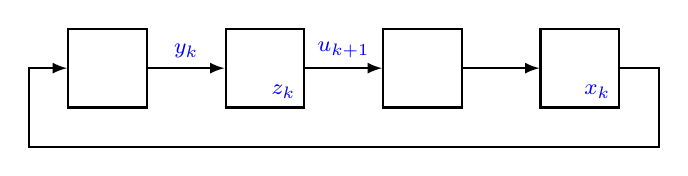
\begin{tikzpicture}
    % Blocks
    \node[draw, rectangle, minimum width = 1cm, minimum height = 1 cm, thick] (s) at (0,0) {$\sensor$};
    \node[draw, rectangle, minimum width = 1cm, minimum height = 1 cm, thick] (c) at (2,0) {$\ctrler$};
    \node[draw, rectangle, minimum width = 1cm, minimum height = 1 cm, thick] (a) at (4,0) {$\actuator$};
    \node[draw, rectangle, minimum width = 1cm, minimum height = 1 cm, thick] (p) at (6,0) {$\plant$};

    \node[anchor=south east, font=\footnotesize, blue] (z) at (c.south east) {$z_k$};
    \node[anchor=south east, font=\footnotesize, blue] (x) at (p.south east) {$x_k$};

    % Arrows
    \draw[->, thick] (s) -- node[above, blue, font=\footnotesize] {$y_k$} (c.west);
    \draw[->, thick] (c) -- node[above, blue, font=\footnotesize] {$u_{k+1}$} (a.west);
    \draw[->, thick] (a) -- (p.west);
    \draw[->, thick] (p.east) -| (7, -1) -| (-1, 0) -- (s.west);
\end{tikzpicture}
 
    \caption{Block diagram representing the interconnection of different components in a control system. The controller $\ctrler$ receives input from the sensor $\sensor$ and sends data to the actuator $\actuator$, which in turn acts on the plant $\plant$.}
    \label{fig:scheme}
\end{figure}
Starting from the \emph{sensors} $\sensor$, the plant is sampled at discrete time instants $k$.
The controller $\ctrler$ then polls the sensor channel for the latest sampled measurement signal to use in the calculation of the new control command $u_k$.
When the new control command is computed, the controller stores it in memory before sending it to the \emph{actuator} $\actuator$ at the beginning of the next control iteration.
Finally, the actuator acts upon the plant $\plant$, based on the command it received from the controller.

\subsection{Fault Model}%
\label{sec:impl}%
%
As anticipated, we aim at devising a stochastic analysis that determines the stability of the closed-loop system in the presence of faults.
We assume that three components in the real-time control system can experience faults (possibly simultaneously)
%
\begin{enumerate*}[label=(\roman*)]
    \item the \emph{sensor channel}, that transmits information between the sensor $\sensor$ and controller $\ctrler$,
    \item the \emph{control task}, that executes the algorithm of the controller $\ctrler$, and 
    \item the \emph{actuator channel}, that allows the controller $\ctrler$ to communicate with the actuator $\actuator$.
\end{enumerate*}
%
We provide a brief review of what can cause problems for both the controller and the input/output (IO) channels, together with some common implementation details.

\subsubsection*{Control Task and Overruns}
Controllers $\ctrler$ should periodically calculate a control signal based on~\eqref{eq:ctrler}. They are generally implemented in \emph{control tasks}, i.e., periodic tasks with implicit deadlines.
A typical implementation is the following.
\begin{lstlisting}[label=lst:control-job,caption={Typical control algorithm execution.}]
while True:
    y = read_sensor_ch()
    u, z = compute_control(y, z)
    sleep_until(next_activation)
    send_actuator_ch(u)
\end{lstlisting}
The code in Listing~\ref{lst:control-job} performs the following operations
\begin{enumerate*}[label=(\roman*)]
    \item it samples the current plant measurements in \texttt{y} using the sensor $\sensor$ (via the function \texttt{read\_sensor\_ch}),
    \item it calculates and stores in memory the next control signal \texttt{u} and the controller's updated state \texttt{z} (via \texttt{compute\_control}),
    \item it sleeps until the next activation (via \texttt{sleep\_until}), and
    \item it sends the control commands to the actuators $\actuator$ (via \texttt{send\_actuator\_ch}).
\end{enumerate*}

For the control task, each iteration of the loop in Listing~\ref{lst:control-job} is a new \emph{job}, and the $k$-th iteration corresponds to the job $j_k$.
The control job $j_k$ is \emph{released} at time $a_k = k\,\Ts$, where $\Ts$ is the \emph{period} of the control task.
The objective of each job is to complete its execution before its corresponding \emph{deadline} $d_k = a_k + \Ts = (k+1)\,\Ts$.
We denote with $f_k$ the time instant in which the control task \emph{completes} the execution of job $j_k$.
Ideally, $f_k \leq d_k$.

If $f_k > d_k$, job $j_k$ experiences an \emph{overrun}, or a deadline miss.
Overruns can be caused by many different factors, like preemption from higher priority tasks and interrupts~\cite{Stankovic:1995}, timeouts due to long wait times on the sensor channel~\cite{Ohlin:2006}, and cache misses that introduce delays in accessing the controller's stored variables~\cite{Wang:2012}.

Regardless of what caused the overrun, the scheduler needs to react.
In the literature~\cite{Cervin:2005}, mainly three simple \emph{deadline overrun strategies} have been considered
%
\begin{enumerate*}[label=(\roman*)]
    \item \tK{} -- i.e., \emph{killing} the job that overran its deadline (and releasing a new one), rolling back any (possibly partial) change performed by the job that missed its deadline, thus reverting the internal task state variables to their original value,
    \item \tS{} -- i.e., letting the job continue its execution, \emph{skipping} the subsequent job releases, until the current one has completed its execution, or
    \item \tQ{} -- i.e., combining the two, and letting the job continue its execution but at the same time \emph{queueing} the subsequent job executions.
\end{enumerate*}
%
In the case of \tS{} and \tQ{}, the job that continues executing operates on outdated data.
On the contrary, \tK{} allows the task to always work with fresh data, with the risk of throwing away near-completed computations.
The \tQ{} strategy has been shown to create chain effects which can severely damage control systems~\cite{Cervin:2005, Maggio:2020}, hence in this paper we only consider \tK{} and \tS{} as viable strategies.

\subsubsection*{Sensor Channel Dropouts}
Control systems rely on communication interfaces between the sensors/actuator and the controller code itself (i.e., the sensor and actuator channels).
A significant amount of research, including~\cite{Ling:2002, Linsenmayer:2017, Kauer:2014, Goswami:2014}, analysed the problem of control system's stability and performance when subject to sensor packet losses.
Losing packets over the sensor channel can lead to the controller not updating the control command, using old measurement data, or even missing job deadlines due to prolonged waiting times.
In these cases, the time in between two sampling instants is time-varying, and control design strategies can be applied to optimise the control system performance~\cite{Ghosh:2018, Schinkel:2002}.
However, this work does not take into account that packet losses could be combined with deadline overruns.

Furthermore, in the code snippet shown in Listing~\ref{lst:control-job}, there is no indication of how the control task reacts to sensor packet losses.
In classical controller implementations, if no sensor packet is received within a given time limit (typically a fraction of the deadline), the function \texttt{read\_sensor\_ch} \emph{times out}, and the control algorithm can perform one of the following two actions
%
\begin{enumerate*}[label=(\roman*)]
    \item \emph{continue} its execution, without updating the value of \texttt{y}, thus using the previous received sensor value, or
    \item \emph{avoid} executing the remaining instructions, terminating the computation early.
\end{enumerate*}

The choice of continuing or avoiding is highly dependent on the system dynamics.
Assuming that packet losses are relatively uncommon and the control period is typically short, using continue is advantageous.
In fact, if a packet is lost, it is still likely that the previous value reported by the sensor is a reasonable approximation of the physical environment.
We emphasise that continuing the execution is equivalent to the case when the controller does not directly poll the sensor channel, but rather reads the most recently received sensor value from memory (where it was stored by a receiver task).
On the other hand, avoiding the execution of the remaining instructions also prevents the controller from evolving its state \texttt{z} and control signal \texttt{u} in a possibly unsafe direction.
Listings~\ref{lst:continue} and~\ref{lst:pass} show more realistic versions of Listing~\ref{lst:control-job} for the continue and avoid cases.

\begin{lstlisting}[label=lst:continue,caption={Control code execution when the control computation is continued if the sensor reading function \texttt{read\_sensor\_ch} results in a timeout.}]
while True:
    y, tout_triggered = read_sensor_ch(tout_seconds)
    if tout_triggered:
        y = y_old
    u, z = compute_control(y, z)
    y_old = y
    sleep_until(next_activation)
    send_actuator_ch(u)
\end{lstlisting}
%
\newpage
\begin{lstlisting}[label=lst:pass,caption={Control code execution when the control computation is avoided if the sensor reading function \texttt{read\_sensor\_ch} results in a timeout.}]
while True:
    y, tout_triggered = read_sensor_ch(tout_seconds)
    if not tout_triggered:
        u, z = compute_control(y, z)
    sleep_until(next_activation)
    send_actuator_ch(u)
\end{lstlisting}

In Listings~\ref{lst:continue} and~\ref{lst:pass}, when \texttt{tout\_seconds} time units have passed without completion, the receive function \texttt{read\_sensor\_ch} sets the variable \texttt{tout\_triggered} to true.
In Listing~\ref{lst:continue}, the control algorithm continues executing its instructions using the old sensor value \texttt{y\_old}, i.e., the controller's internal state \texttt{z} will be updated and a new control command \texttt{u} will be sent to the actuators.
In Listing~\ref{lst:pass}, the control algorithm will not be run, i.e., the internal state \texttt{z} and the control command \texttt{u} are kept constant.

\subsubsection*{Actuator Channel Dropouts}
Packet losses on the actuator channel have not been studied as thoroughly as their sensor counterpart.
The reason likely comes from the fact that the actuator response is typically hardware-dependant and difficult to detect and compensate in the control algorithm.
If the actuator does not receive a new control command when it is expecting one, it defaults to a value dependent on the \emph{actuation mode}.
The actuation mode has received more attention, with different degradation or stabilising actuation policies being proposed~\cite{Ma:2018}.
However, the most common approaches involve either \tH{}ing the last received control command (i.e., $u_{k+1} = u_k$) or \tZ{}ing the output (i.e., $u_{k+1}=0$).
Similarly to choosing between continue and avoid, the choice of actuation mode is non-trivial and generally depend on the control system dynamic~\cite{Schenato:2009, Vreman:2021}.

\subsection{Problem Formulation}%
\label{sec:prob}%
Many different analysis frameworks have been proposed to evaluate the computational robustness to packet loss and deadline overruns of controllers~\cite{Ghosh:2018, Maggio:2020, Linsenmayer:2017, Heemels:2011}.
However, these analyses have two major shortcomings:
\begin{enumerate*}[label=(\roman*)]
    \item they are developed in isolation, and do not combine the presence of potential problems both in the computation and in the IO channels, and
    \item they rely on knowledge about the occurrence of events like deadline overruns or packet losses.
\end{enumerate*}
In fact, recent works on computational overruns~\cite{Maggio:2020, Linsenmayer:2017} rely on the weakly-hard task model~\cite{Bernat:2001} to constraint the sequence of deadline overruns; and recent work like~\cite{Ghosh:2018} are on the contrary working on the assumption that packet losses are detected and counteracted at the control level.
However, typical methods for deriving bounds on both packet losses and deadline overruns are probabilistic; for example, estimating the probability that a specific task in a system will overrun its deadline when a particular scheduling algorithm is employed~\cite{Chen:2019, Bruggen:2021}.

This paper aims at providing a control-theoretical analysis for how the closed-loop system robustness is affected by stochastic packet losses (on sensor and actuator channels), deadline overruns, and a combination thereof.
Furthermore, we want to devise an analysis method that benefits from the state-of-the-art results on fault occurrence estimation in real-time systems implementations~\cite{Chen:2019, Bruggen:2021}.
We assume to receive, as input, probabilities $p_c$, $p_s$, and $p_a$.
These represent respectively the probability of the control task missing its deadline, the probability of a failure on the sensor channel and the probability of a packet loss on the actuator channel.
The analysis provides -- as output -- a certificate that specifies that the system does or does not satisfy a stochastic stability requirement.
If the certificate verifies the stochastic stability of the closed-loop system, then the average value $\E{\tilde{x}_k}$ of the system state $\tilde{x}_k$, introduced in Equation~\eqref{eq:clsys}, converges to a given value and its standard deviation converges to zero.
This allows us to validate the control system implementation behaviour in the presence of undesirable faults.


\section{Analysis}
\label{sec:anl}
Our analysis of the closed-loop system subject to IO channel dropouts and deadline overruns is based on the theory of Markov Jump Linear Systems~\cite{Costa:2005}.
These systems combine the dynamics of the closed-loop system and the transition probabilities of faults and errors.
In Section~\ref{sec:prel} we provide some preliminary definitions and in Section~\ref{sec:dynamics} we derive the control system dynamics when (possibly simultaneously) deadline overruns, sensor data loss, and actuator data loss occur.
In Section~\ref{sec:mc} we present the Markov chain that describes the probabilistic evolution of the discrete state of the system.
Finally, in Section~\ref{sec:mjls} we summarise and apply the Markov Jump Linear Systems theory to the closed-loop system, obtaining the stochastic stability certificates.
Note that the concept of \emph{state} differs between Markov and control theory.
With the word \emph{state} we denote the dynamical system's state vector $\tilde{x}_k$, whilst the information encoded by a sequence of events including IO channel dropouts and computational overruns is referred to as the \emph{discrete state}.

\subsection{Event Outcomes}%
\label{sec:prel}%

Equation~\eqref{eq:nom} presented the dynamical model of the closed-loop system and the closed-loop state matrix $\clmat$ in nominal conditions, i.e., in the absence of faults.
However, as discussed in Section~\ref{sec:prb}, the system dynamics are heavily impacted by whether the controller misses a control computation or experiences a packet loss on either of the communication channels.
To analyse the system dynamics, we define the \emph{outcome set} $\Sigma$ for the transmission on IO channels and the computation of the controller.
\begin{definition}[IO Channel Outcome Sets]%
    \label{def:comm}%
    We denote the set of outcomes that each packet on the sensor and actuator channels can experience by $\osets = \oseta = \left\{ \cF, \cT \right\}$:
    \begin{itemize}
        \item $\cF$: represents a lost packet, and
        \item $\cT$: represents a successfully delivered packet.
    \end{itemize}
\end{definition}
%
Trivially, the outcome of each packet transmission is a binary event where either:
\begin{enumerate*}[label=(\roman*)]
    \item the packet is successfully received (\cT), or
    \item the packet is lost somewhere along its route (\cF).
\end{enumerate*}
Since the contents of the packet (e.g., measurement data from the sensors or control commands to the actuators) is irrelevant to whether the packet is lost or not, the same outcome notation is used for both $\osets$ and $\oseta$.

Unlike the IO channels, the outcome of a control job's computation is not necessarily a binary event.
In particular, the overrun strategy employed by the scheduler determines the outcome set.
We now define the control task outcome sets (for one execution interval, i.e., for one \emph{control period}) both for the \tK{} and for the \tS{} strategy.
%
\begin{definition}[Computational Outcome Set - \tK{}]%
    \label{def:kill}%
    We denote the set of outcomes that a control job can experience in each control period when the scheduler adopts the \tK{} strategy by $\osetck = \left\{ \cM, \cH \right\}$.
    \begin{itemize}
        \item $\cM$: a job is released, but no job is completed, 
        \item $\cH$: a job is both released and completed.
    \end{itemize}
\end{definition}
%
\begin{definition}[Computational Outcome Set - \tS{}]%
    \label{def:skip}%
    We denote the set of outcomes that a control job can experience in each control period when the scheduler adopts the \tS{} strategy by $\osetcs = \left\{ \cM, \cN, \cH, \cR \right\}$.
    \begin{itemize}
        \item $\cM$: a new control job is released but no job is completed,
        \item $\cN$: no job is either released or completed, 
        \item $\cH$: a new control job is both released and completed,
        \item $\cR$: no job is released, but a job (that was released in a previous period) is completed.
    \end{itemize}
\end{definition}
%

For both \tK{} and \tS{}, each control period contains \emph{at most} one activated and one completed job.
The main difference comes from the \tK{} strategy terminating every job that overrun its corresponding deadline, i.e., each control period contains a new control job being released and activated.
Thus, the outcome set $\osetck$ consist of only two outcomes: a job being completed or a job not being completed.
On the other hand, the \tS{} strategy encompasses more diverse outcomes.
For instance, the outcomes $\cM$ and $\cN$ both encode an overrun deadline; but $\cM$ represent the start of a control computation while $\cN$ correspond to its continuation.
Finally, $\cR$ is used to identify the \emph{late completion} of a job, i.e., a \emph{recovery hit}.
The occurrence of $\cR$ and $\cN$ impose constraints on the outcome ordering.
We note that if we use the \tS{} overrun strategy, there is a natural valid order between the job outcomes.
The following constraint enforces that a sequence of job outcomes is valid, i.e., it can be produced by a control task.
%
\begin{rule_}%
    \label{rule:1}%
    For a sequence of job outcomes under the \tS{} overrun strategy, it holds that: 
    \begin{itemize}
        \item both $\cM$ and $\cH$ are restricted to directly follow an $\cH$ or $\cR$,
        \item an $\cN$ can only follow an $\cM$, and
        \item an $\cR$ may only directly follow an $\cN$ or $\cM$.
    \end{itemize}
\end{rule_}

\subsection{Closed-Loop System Dynamics}%
\label{sec:dynamics}%

From Definitions~\ref{def:comm}-\ref{def:skip}, the closed-loop system dynamics' evolution in time can be fully derived as (with initial state $\tilde{x}_0$):
%
\begin{equation}
    \label{eq:cl-dynamics} 
    \tilde x_{k+1} = \clmat_{sca}\, \tilde x_k.
\end{equation}
%
As for Equation~\eqref{eq:clsys}, $\tilde x_k$ is the closed-loop state vector and $\clmat_{sca}$ is the closed-loop system matrix.
The system dynamics does however depend on the outcome realisations, i.e., $s \in \osets$, $a \in \oseta$, and $c \in \osetc{\bullet}$ (where $\bullet$ is either $\Kill$ or $\Skip$).
If a fault occurs, the closed-loop system's evolution will deviate from the nominal behaviour.
As an example, the closed-loop system matrix $\clmat_{\cT\cH\cT}$ would correspond to a control job receiving the sensor message, completing its algorithm execution in the same period as it was released, and the actuators would successfully receive the new control command.
Trivially, $\clmat_{\cT\cH\cT}$ correspond to the nominal behaviour from Equation~\eqref{eq:nom}.
Instead, if an actuator packet would be lost, the control command sent to the plant would depend on the actuator mode.
Therefore, the closed-loop system would evolve according to $\clmat_{\cT\cH\cF}$.

Note that in each control period the system experiences a new realisation of the outcome sets, i.e., the closed-loop system matrix $\clmat_{sca}$ can switch every control period.
The resulting dynamics is generally called a \emph{switching system}.
Since the closed-loop dynamics is no longer consistent between periods, the stability criterion presented in~\eqref{eq:schur} cannot be used to assess the stability of the system, and we need to resort to a probabilistic stability result, presented in Section~\ref{sec:mjls}.

As discussed in Section~\ref{sec:prb}, the system dynamics change with respect to
\begin{enumerate*}[label=(\roman*)]
    \item the overrun strategy,
    \item the actuation mode, and
    \item the choice of timeout strategy.
\end{enumerate*}
In this paper, we focus on the stability analysis for the continue case, as the possible \emph{outcome configurations} (i.e., combinations of $s$, $c$, and $a$) for the avoid case are included in the set of outcome configurations for continue, making the analysis simpler in the avoid case.\footnote{Additionally, \emph{continue} also cover the case where the controller reads sensor data directly from a memory register instead of polling the sensor channel.}
In the continue case, we provide a stability analysis for both actuation modes (i.e., \tZ{} or \tH{}) and both overrun strategies (i.e., \tK{} or \tS{}).
The difference between \tZ{} and \tH{} result in variations of the closed-loop matrices, and is encoded using the symbol $\Delta_\actuator$, described later.
However, the difference between using \tK{} and \tS{} fundamentally changes the structure of the outcome set of the control jobs changes.
Hence, we need to analyse the \tK{} and \tS{} cases separately.

\subsubsection*{\tK{}:}
%
When a fault is experienced (deadline overrun or packet loss), the physical state of the plant $x_k$ continue its normal evolution.
However, the closed-loop will not behave according to its design specifications.
In case $j_k$ overruns its deadline, its execution is terminated and the controller's states are rolled back, i.e., $z_{k+1} = z_k$.
Furthermore, when $j_k$ overruns its deadline \emph{or} the actuator channel experiences a packet loss, the control command defaults to a value that depends on the actuation mode, i.e., $u_{k+1} = u_k$ if the actuation mode is \tH{}, and $u_{k+1} = 0$ if the actuation mode is \tZ{}.
On the contrary, if a sensor packet is not received, the control algorithm computes a new control command and updates the controller's internal state, using outdated sensor measurements.

To properly describe the closed-loop behaviour under continue and \tK{}, we define the closed-loop state vector 
%
$\tilde x_k^{\Kill} = [ x_k^\T{}, z_k^\T{}, u_k^\T{}, \hat y_{k-1}^\T{} ]^\T{}.$
%
The introduced auxiliary state $\hat y_{k-1}$ records the old sensor value, that is used if \texttt{read\_sensor\_ch} times out (see Listing~\ref{lst:continue}).

The set of closed-loop matrices describing the system behaviour for the different outcome configurations is 
%%% KILL
%\begin{figure*}[ht]
%    \centering\scriptsize
    \begin{equation}
        \label{eq:cont-kill} 
        \begin{matrix}
            \underbrace{\begin{bmatrix}
                A  & 0 & B & 0 \\
                GC & F & GD & 0 \\
                KC & H & KD & 0 \\
                C & 0 & D & 0 \\
            \end{bmatrix}}_{\clmat_{\cT\cH\cT}^{\Kill}} &
            \underbrace{\begin{bmatrix}
                A & 0 & B & 0 \\
                GC & F & GD & 0 \\
                0 & 0 & \Delta_\actuator & 0 \\
                C & 0 & D & 0
            \end{bmatrix}}_{\clmat_{\cT\cH\cF}^{\Kill}} &
            \underbrace{\begin{bmatrix}
                A & 0 & B & 0 \\
                0 & I & 0 & 0 \\
                0 & 0 & \Delta_\actuator & 0 \\
                C & 0 & D & 0
            \end{bmatrix}}_{\clmat_{\cT\cM\cT}^{\Kill}} &
            \underbrace{\begin{bmatrix}
                A & 0 & B & 0 \\
                0 & I & 0 & 0 \\
                0 & 0 & \Delta_\actuator & 0 \\
                C & 0 & D & 0
            \end{bmatrix}}_{\clmat_{\cT\cM\cF}^{\Kill}} \\[4em]
            \underbrace{\begin{bmatrix}
                A & 0 & B & 0 \\
                0 & F & 0 & G \\
                0 & H & 0 & K \\
                0 & 0 & 0 & I
            \end{bmatrix}}_{\clmat_{\cF\cH\cT}^{\Kill}} &
            \underbrace{\begin{bmatrix}
                A & 0 & B & 0 \\
                0 & F & 0 & G \\
                0 & 0 & \Delta_\actuator & 0 \\
                0 & 0 & 0 & I
            \end{bmatrix}}_{\clmat_{\cF\cH\cF}^{\Kill}} &
            \underbrace{\begin{bmatrix}
                A & 0 & B & 0 \\
                0 & I & 0 & 0 \\
                0 & 0 & \Delta_\actuator & 0 \\
                0 & 0 & 0 & I
            \end{bmatrix}}_{\clmat_{\cF\cM\cT}^{\Kill}} &
            \underbrace{\begin{bmatrix}
                A & 0 & B & 0 \\
                0 & I & 0 & 0 \\
                0 & 0 & \Delta_\actuator & 0 \\
                0 & 0 & 0 & I
            \end{bmatrix}}_{\clmat_{\cF\cM\cF}^{\Kill}}
        \end{matrix}.
    \end{equation}%
%\end{figure*}
%
Each outcome ($s$, $c$, and $a$) has $2$ possible configurations in the \tK{} case.
Hence, there are $2^3 = 8$ possible $sca$, where $s \in \osets$, $c \in \osetck$, and $a \in \oseta$.
As anticipated, the symbol $\Delta_\actuator$ in Equation~\eqref{eq:cont-kill} is used to distinguish the actuator mode, and is either $\Delta_\actuator = I$ for the \tH{} mode or $\Delta_\actuator = 0$ for the \tZ{} mode.
The variable $\hat y_k$ is not updated for $s = \cF$, i.e., $\hat y_k = \hat y_{k-1}$.
Additionally, some matrices are identical (e.g., $\clmat^{\Kill}_{\cT\cM\cT}=\clmat^{\Kill}_{\cT\cM\cF}$ and $\clmat^{\Kill}_{\cF\cM\cT}=\clmat^{\Kill}_{\cF\cM\cF}$), highlighting for example that in case of \tK{} when the computation does not complete, receiving or not receiving the actuator signal is irrelevant for the system evolution.

\subsubsection*{\tS{}:}
Similarly to the \tK{} case, when the computation mode for overruns is set to \tS{}, the physical states $x_k$ continue their evolution.
However, in contrast to the \tK{} overrun strategy, when a job $j_k$ overruns its deadline, the job is allowed to continue its execution, and no subsequent jobs are released until $j_k$ completes its execution.

As an example, assume that job $j_k$, released at time $a_k$, finishes its execution at time $f_k = a_k + 3.7\,\Ts$.
In this case, three subsequent jobs are skipped.
During the three control periods in which $j_k$ is still pending completion, no new job is released and the actuator outputs a control command that is in line with the actuation mode, either \tH{} or \tZ{}.
When $j_k$ completes its execution, the controller state is updated and the control command is computed using the sensor value that was retrieved at time $a_k$, i.e., depending on whether the sensor packet at time $a_k$ was received or not.
In this case, the new control signal is sent to the actuator at the end of the control period, at time instant $a_k+4\,\Ts$.

The closed-loop state vector for the continue and \tK{} case can be reused to describe the system evolution of the continue and \tS{} case, i.e., $\tilde x_k^{\Skip} = [ x_k^\T{}, z_k^\T{}, u_k^\T{}, \hat y_{k-1}^\T{} ]^\T{}$.
Intuitively, there are $16$ possible outcome configurations since $\osetcs{}$ contains four outcomes rather than two, i.e., $2^2\cdot 4=16$.
Using $\Delta_\actuator = I$ and $\Delta_\actuator = 0$ to indicate, respectively, the \tH{} and \tZ{} actuation mode, the closed-loop matrices are
%%% SKIP
%\begin{figure*}[ht]
%\centering\scriptsize
    \begin{equation}
        \label{eq:cont-skip} 
        %\resizebox{0.955\textwidth}{!}{$%
            \begin{matrix}
                \underbrace{\begin{bmatrix}
                    A  & 0 & B & 0 \\
                    GC & F & GD & 0 \\
                    KC & H & KD & 0 \\
                    C & 0 & D & 0 \\
                \end{bmatrix}}_{\clmat_{\cT\cH\cT}^{\Skip}} &
                \underbrace{\begin{bmatrix}
                    A & 0 & B & 0 \\
                    GC & F & GD & 0 \\
                    0 & 0 & \Delta_\actuator & 0 \\
                    C & 0 & D & 0
                \end{bmatrix}}_{\clmat_{\cT\cH\cF}^{\Skip}} &
                \underbrace{\begin{bmatrix}
                    A & 0 & B & 0 \\
                    0 & I & 0 & 0 \\
                    0 & 0 & \Delta_\actuator & 0 \\
                    C & 0 & D & 0
                \end{bmatrix}}_{\clmat_{\cT\cM\cT}^{\Skip}} &
                \underbrace{\begin{bmatrix}
                    A & 0 & B & 0 \\
                    0 & I & 0 & 0 \\
                    0 & 0 & \Delta_\actuator & 0 \\
                    C & 0 & D & 0
                \end{bmatrix}}_{\clmat_{\cT\cM\cF}^{\Skip}} \\[4em]
                \underbrace{\begin{bmatrix}
                    A & 0 & B & 0 \\
                    0 & I & 0 & 0 \\
                    0 & 0 & \Delta_\actuator & 0 \\
                    0 & 0 & 0 & I
                \end{bmatrix}}_{\clmat_{\cT\cN\cT}^{\Skip}} &
                \underbrace{\begin{bmatrix}
                    A & 0 & B & 0 \\
                    0 & I & 0 & 0 \\
                    0 & 0 & \Delta_\actuator & 0 \\
                    0 & 0 & 0 & I
                \end{bmatrix}}_{\clmat_{\cT\cN\cF}^{\Skip}} &
                \underbrace{\begin{bmatrix}
                    A & 0 & B & 0 \\
                    0 & I & 0 & 0 \\
                    0 & 0 & \Delta_\actuator & 0 \\
                    0 & 0 & 0 & I
                \end{bmatrix}}_{\clmat_{\cF\cN\cT}^{\Skip}} &
                \underbrace{\begin{bmatrix}
                    A & 0 & B & 0 \\
                    0 & I & 0 & 0 \\
                    0 & 0 & \Delta_\actuator & 0 \\
                    0 & 0 & 0 & I
                \end{bmatrix}}_{\clmat_{\cF\cN\cF}^{\Skip}} \\[4em]
                \underbrace{\begin{bmatrix}
                    A & 0 & B & 0 \\
                    0 & F & 0 & G \\
                    0 & H & 0 & K \\
                    0 & 0 & 0 & I
                \end{bmatrix}}_{\clmat_{\cT\cR\cT}^{\Skip}} &
                \underbrace{\begin{bmatrix}
                    A & 0 & B & 0 \\
                    0 & F & 0 & G \\
                    0 & H & 0 & K \\
                    0 & 0 & 0 & I
                \end{bmatrix}}_{\clmat_{\cF\cR\cT}^{\Skip}} &
                \underbrace{\begin{bmatrix}
                    A & 0 & B & 0 \\
                    0 & F & 0 & G \\
                    0 & 0 & \Delta_\actuator & 0 \\
                    0 & 0 & 0 & I
                \end{bmatrix}}_{\clmat_{\cT\cR\cF}^{\Skip}} &
                \underbrace{\begin{bmatrix}
                    A & 0 & B & 0 \\
                    0 & F & 0 & G \\
                    0 & 0 & \Delta_\actuator & 0 \\
                    0 & 0 & 0 & I
                \end{bmatrix}}_{\clmat_{\cF\cR\cF}^{\Skip}}
\end{matrix}
\end{equation}
\begin{equation*}
        \label{eq:cont-skip-2} 
            \begin{matrix}
                \underbrace{\begin{bmatrix}
                    A & 0 & B & 0 \\
                    0 & F & 0 & G \\
                    0 & H & 0 & K \\
                    0 & 0 & 0 & I
                \end{bmatrix}}_{\clmat_{\cF\cH\cT}^{\Skip}} &
                \underbrace{\begin{bmatrix}
                    A & 0 & B & 0 \\
                    0 & F & 0 & G \\
                    0 & 0 & \Delta_\actuator & 0 \\
                    0 & 0 & 0 & I
                \end{bmatrix}}_{\clmat_{\cF\cH\cF}^{\Skip}} &
                \underbrace{\begin{bmatrix}
                    A & 0 & B & 0 \\
                    0 & I & 0 & 0 \\
                    0 & 0 & \Delta_\actuator & 0 \\
                    0 & 0 & 0 & I
                \end{bmatrix}}_{\clmat_{\cF\cM\cT}^{\Skip}} &
                \underbrace{\begin{bmatrix}
                    A & 0 & B & 0 \\
                    0 & I & 0 & 0 \\
                    0 & 0 & \Delta_\actuator & 0 \\
                    0 & 0 & 0 & I
                \end{bmatrix}}_{\clmat_{\cF\cM\cF}^{\Skip}} &
            \end{matrix}.
        %$}%
    \end{equation*}
%\end{figure*}
%
%

When $c=\cR$ or $c=\cN$, the sensor packet's outcome is irrelevant for the system dynamics.
This follows since the control task does not poll the sensor channel for packets if it is still executing the body of the control algorithm (unless its outcome is $\cM$, since it is the first period that experiences an overrun).
Again, note that many matrices are identical:
%\begin{equation*}
%    \clmat^{\Skip}_{\cF\cM\cT} = \clmat^{\Skip}_{\cF\cM\cF};\quad \clmat^{\Skip}_{\cT\cM\cT} = \clmat^{\Skip}_{\cT\cM\cF};\quad \clmat^{\Skip}_{\cT\cN\cT} = \clmat^{\Skip}_{\cT\cN\cF} = \clmat^{\Skip}_{\cF\cN\cT} = \clmat^{\Skip}_{\cF\cN\cF};\quad \clmat^{\Skip}_{\cF\cR\cT} = \clmat^{\Skip}_{\cT\cR\cT};\quad \clmat^{\Skip}_{\cF\cR\cF} = \clmat^{\Skip}_{\cT\cR\cF},
%\end{equation*}
\begin{align*}
    \clmat^{\Skip}_{\cF\cM\cT} &= \clmat^{\Skip}_{\cF\cM\cF},\quad \clmat^{\Skip}_{\cT\cM\cT} = \clmat^{\Skip}_{\cT\cM\cF} \\
    \clmat^{\Skip}_{\cT\cN\cT} &= \clmat^{\Skip}_{\cT\cN\cF} = \clmat^{\Skip}_{\cF\cN\cT} = \clmat^{\Skip}_{\cF\cN\cF} \\
    \clmat^{\Skip}_{\cF\cR\cT} &= \clmat^{\Skip}_{\cT\cR\cT},\quad \clmat^{\Skip}_{\cF\cR\cF} = \clmat^{\Skip}_{\cT\cR\cF},
\end{align*}
which can be used to simplify the stability analysis below.

While we introduced the dynamical system change associated with different events (i.e., with different combinations of sensor channel $s$, actuator channel $a$, and computational outcome $c$), so far we only described the deterministic evolution of the system.
Provided that a specific set of events occurs during the evolution of the discrete part of our problem, the system behaviour is deterministic.
However, the discrete state evolution of the closed-loop system is probabilistic and depends on the outcome of $s$, $c$, and $a$, which is here expressed via a Markov process.

\subsection{Markov Chain}%
\label{sec:mc}%

To take the discrete state evolution into account, we introduce a Markov chain.
A Markov chain is a mathematical model for a stochastic process that describes a sequence of events or states, where the probability of transitioning from one state to another depends only on the current state and not on any previous states.

\begin{definition}[Markov Chain]
    A Markov chain is defined by:
    \begin{enumerate}[label=(\roman*)]
        \item A set $\Theta$ of $N$ possible states, $\Theta = \{ v_1, v_2, \dots, v_N \}$,
        \item A transition probability matrix $\Pi$, where the element $\Pi_{i, j}$ is the probability of transitioning from state $v_i$ to state $v_j$, for all $i,j \in \{ 1,2, \dots ,N \}$,
        \item The Markov property, which states that the probability of transitioning to a future state depends only on the current state and not on any past states.
    \end{enumerate}
    The transition probability matrix $\Pi$ must satisfy the following two conditions:
    \begin{enumerate}[label=(\roman*)]
        \itemsep1pt
        \item $\Pi_{i, j} \geq 0, \, \forall i,j \in \{1,2,...,N\}$,
        \item $\sum^{N}_{j=1} \Pi_{i, j} = 1, \forall i \in \{1,2,...,N\}$.
    \end{enumerate}
\end{definition}

In our case, each state of the Markov chain represents an element of the set of outcomes, and directly maps to one of the matrices that govern the physical evolution of the system.
The transition probabilities of the Markov chain depend on respectively
\begin{enumerate*}[label=(\roman*)]
    \item $p_s$ -- the probability of not receiving sensor data correctly,
    \item $p_c$ -- the probability of not completing the calculation of the control signal within one period, and
    \item $p_a$ -- the probability of not receiving the actuator data correctly.
\end{enumerate*}
As an example, the probability that in one period we transition to the state in which no faults occurred, $s=\cT$, $c=\cH$, $a=\cT$ is $(1-p_s)\,(1-p_c)\,(1-p_a)$.
In such a discrete state, the discrete-time dynamics evolve according to $\clmat_{\cT\cH\cT}$.
For compactness, we use the notation $1_x$ to denote $(1-p_x)$, e.g., $1_s = (1-p_s)$.

\subsubsection*{\tK{}:}
For the \tK{} case, in principle there are $8$ states in the Markov chain (stemming from the $8$ possible matrices), but the equivalence between two pairs of matrices reduces the discrete states in which the system can be found to $6$, corresponding to the closed-loop matrices $\clmat^{\Kill}_{\cT\cH\cT}$, $\clmat^{\Kill}_{\cF\cH\cT}$, $\clmat^{\Kill}_{\cT\cH\cF}$, $\clmat^{\Kill}_{\cF\cH\cF}$, $\clmat^{\Kill}_{\cF\cM\cX}$ and $\clmat^{\Kill}_{\cT\cM\cX}$, where $\cX$ indicates that the outcome is irrelevant for this specific case.
The Markov chain for the \tK{} strategy is encoded in the transition probability matrix
\begin{equation}
\label{eq:pikill}
\Pi^{\Kill} = \begin{bmatrix}
        1_s1_c1_a & p_s1_c1_a & 1_s1_cp_a & p_s1_cp_a & p_sp_c & 1_sp_c \\
        1_s1_c1_a & p_s1_c1_a & 1_s1_cp_a & p_s1_cp_a & p_sp_c & 1_sp_c \\
        1_s1_c1_a & p_s1_c1_a & 1_s1_cp_a & p_s1_cp_a & p_sp_c & 1_sp_c \\
        1_s1_c1_a & p_s1_c1_a & 1_s1_cp_a & p_s1_cp_a & p_sp_c & 1_sp_c \\
        1_s1_c1_a & p_s1_c1_a & 1_s1_cp_a & p_s1_cp_a & p_sp_c & 1_sp_c \\
        1_s1_c1_a & p_s1_c1_a & 1_s1_cp_a & p_s1_cp_a & p_sp_c & 1_sp_c \\
\end{bmatrix}.
\end{equation}

In $\Pi^{\Kill}$, the rows correspond to the following dynamical system matrices: $\clmat^{\Kill}_{\cT\cH\cT}$, $\clmat^{\Kill}_{\cF\cH\cT}$, $\clmat^{\Kill}_{\cT\cH\cF}$, $\clmat^{\Kill}_{\cF\cH\cF}$, $\clmat^{\Kill}_{\cF\cM\cX}$, $\clmat^{\Kill}_{\cT\cM\cX}$.
The transition matrix is fully connected, as from each state it is possible to reach any other state.
Also, given the nature of the \tK{} action, every iteration of the control loop is independent, and therefore the probability to reach any state in the Markov chain is the same, regardless of the current state.

\subsubsection*{\tS{}:}
In the \tS{} case, the transition matrix is not fully connected.
In fact, each sequence of outcomes should satisfy Constraint~\ref{rule:1}, enforcing that $\cH$ can only occur after either another $\cH$ or $\cR$.
Also, $\cN$ must directly follow $\cM$, and a $\cR$ can only follow a $\cM$ or $\cN$.
Hence, the transition matrix $\Pi^{\Skip}$ of the Markov chain for the continue and \tS{} case is
\begin{equation}
\label{eq:piskip}
\Pi^{\Skip} = \begin{bmatrix}
            1_s1_c1_a & p_s1_c1_a & 1_s1_cp_a & p_s1_cp_a & p_sp_c & 1_sp_c & 0 & 0 & 0 \\
            1_s1_c1_a & p_s1_c1_a & 1_s1_cp_a & p_s1_cp_a & p_sp_c & 1_sp_c & 0 & 0 & 0 \\
            1_s1_c1_a & p_s1_c1_a & 1_s1_cp_a & p_s1_cp_a & p_sp_c & 1_sp_c & 0 & 0 & 0 \\
            1_s1_c1_a & p_s1_c1_a & 1_s1_cp_a & p_s1_cp_a & p_sp_c & 1_sp_c & 0 & 0 & 0 \\
            0 & 0 & 0 & 0 & 0 & 0 & p_c & 1_c1_a & 1_cp_a \\
            0 & 0 & 0 & 0 & 0 & 0 & p_c & 1_c1_a & 1_cp_a \\
            0 & 0 & 0 & 0 & 0 & 0 & p_c & 1_c1_a & 1_cp_a \\
            1_s1_c1_a & p_s1_c1_a & 1_s1_cp_a & p_s1_cp_a & p_sp_c & 1_sp_c & 0 & 0 & 0 \\
            1_s1_c1_a & p_s1_c1_a & 1_s1_cp_a & p_s1_cp_a & p_sp_c & 1_sp_c & 0 & 0 & 0 \\
\end{bmatrix}.
\end{equation}
In $\Pi^{\Skip}$, the rows correspond to the following dynamical system matrices: $\clmat^{\Skip}_{\cT\cH\cT}$, $\clmat^{\Skip}_{\cF\cH\cT}$, $\clmat^{\Skip}_{\cT\cH\cF}$, $\clmat^{\Skip}_{\cF\cH\cF}$, $\clmat^{\Skip}_{\cF\cM\cX}$, $\clmat^{\Skip}_{\cT\cM\cX}$, $\clmat^{\Skip}_{\cX\cN\cX}$, $\clmat^{\Skip}_{\cX\cR\cT}$, $\clmat^{\Skip}_{\cX\cR\cF}$.
As can be seen for example in the fifth row, a miss can only be followed by either another miss or a recovery hit, i.e., a period in which no new job is released, but a previously released job is completed.
 
The transition probabilities are here treated as independent identically distributed (i.e., iid) random variables.
Typically this is not the case in real systems.
For example, if the sensor packet is lost, the probability of the control task overrunning its deadline likely increases.
It is possible to cast said cases in our analysis framework using the theory of \emph{conditional probabilities}~\cite{Dekking:2006}, i.e., probabilities that depend on the outcome of another event.
This is done by considering vectors of $p_s$, $p_c$, and $p_a$ in which each element represents the possibility of having a given number of faults in the corresponding event outcome, e.g., the second element of $p_c$ represents the probability that the controller overruns in two consecutive periods.
Then it is possible to create a Markov chain that handles every iteration starting from the corresponding state (e.g., the second element of $p_c$ is only used when a first deadline overrun has occurred and the transition matrix has more zeros).
Due to space limitations, we do not enter into details on this matter here.
This is in particular interesting for $p_c$, as a deadline miss that follows another miss is less likely than the first deadline miss to occur when \tS{} is used.

\subsection{Markov Jump Linear Systems Analysis}%
\label{sec:mjls}%

Discrete-Time Markov Jump Linear Systems~\cite{Costa:2005} describe systems that can switch between different linear dynamics based on a finite set of discrete states.
Informally, these systems combine the concepts of (discrete-time) switched linear systems and Markov chains.
The system is subject to stochastic mode transitions described by a probability matrix (that specifies the likelihood of transitioning from one mode to another), i.e., the transition probability matrix of a Markov chain.
%
\begin{definition}[Discrete-Time Autonomous Markov Jump Linear System]%
    \label{def:mjls}%
    A Discrete-Time Autonomous Markov Jump Linear System is a dynamical system (with initial state $\{\tilde{x}_0, \theta_0\}$) of the form
    \begin{equation*}
        \tilde{x}_{k+1} = \clmat_{\theta_k} \tilde{x}_k,\text{  where}
    \end{equation*}
    \begin{enumerate}[label=(\roman*)]
        \item $\clmat_{\theta_k}$ belongs to a set of discrete-time linear state-space models describing the evolution of the continuous dynamics, and
        \item $\{\theta_k\}_k$ is a Markov process, governed by a Markov chain with transition probability matrix $\Pi$.
    \end{enumerate}
\end{definition}
%
In our case, the state-space models are given by the matrices derived in Section~\ref{sec:dynamics} and the Markov chain is the one described in Section~\ref{sec:mc}.

The convergence of Markov Jump Linear Systems can be analysed using different tools, and in particular there are two main notions of stability: \emph{mean stability} and \emph{mean square stability}.
Mean stability corresponds to convergence in probability, while the second notion, mean square stability, corresponds to almost sure convergence.\footnote{Other notions of stability also exist, like stochastic stability and mean square exponential stability. However, if a system is mean square stable it is also mean stochastically stable as well as mean square exponentially stable.}% Almost sure convergence is hence a \emph{stronger} notion of stability.}

Mean stability is an important property for ensuring the robustness and reliability of stochastic systems, as it guarantees that the expected value of the system state will not exhibit unbounded growth over time.
We analyse the expected value of the state $x_k$, i.e., $\mathbb{E}\,[x_k]$, and determine whether it converges to a specific value or not.

\begin{definition}[Mean Stability]%
    The Discrete-Time Autonomous Markov Jump Linear System $\tilde{x}_{k+1} = \clmat_{\theta_k} \tilde{x}_k$ is mean stable if there exists a value $\mu$ such that for every initial state $\{\tilde{x}_0, \theta_0\}$, the expected value of the system state $\mathbb{E}\,[\tilde{x}_k] \to \mu$.
\end{definition}

Mean square stability, on the other hand, analyses not only whether the expected value of the discrete-time system state converges, but also whether its covariance $\mathbb{E}\,[\tilde{x}_k \tilde{x}^\T_k]$ goes to zero; thus, implying \emph{almost sure convergence}, i.e., both the probability of the system state converging and the probability of the state covariance going to zero goes to $1$.

\begin{definition}[Mean Square Stability]%
    The Discrete-Time Autonomous Markov Jump Linear System $\tilde{x}_{k+1} = \clmat_{\theta_k} \tilde{x}_k$ is mean square stable if there exists a value $\mu$ such that for every initial state $\{\tilde{x}_0, \theta_0\}$,
    \begin{equation*}
        \mathbb{E}\,[\tilde{x}_k] \to \mu, \quad \mathbb{E}\,[\tilde{x}_k \tilde{x}^\T_k] \to 0.
    \end{equation*}
\end{definition}
Mean square stability is a desirable property for stochastic systems because it implies mean stability, but also provides more information about the rate of decay of the system's fluctuations.
In particular, it implies that the fluctuations experienced by the system will decay exponentially fast over time.
Mean square stability is closely related to the notion of Shur stability for deterministic systems presented in Equation~\eqref{eq:schur}, and is commonly used in the analysis and design of stochastic control and estimation algorithms.

We want to test that the systems subject to fault are mean square stable.
As extensively discussed in the literature~\cite{Costa:2005}, testing for mean square stability implies calculating the eigenvalues of the operator $\Psi$ that defines the evolution of the Markov Jump Linear System's covariance matrix.
In particular, a Discrete-Time Autonomous Markov Jump Linear System is mean square stable if and only if 
\begin{equation}%
    \label{eq:stab-notion}%
    \begin{matrix}
        \rho\,(\Psi) = \max{\abs{\,\eig{}{\Psi}\,}} < 1 \\
        \Psi = (\Pi^\T \otimes I_{n^2}) \cdot \text{blkdiag}\,(\,\{ \clmat_{i}^\T \otimes \clmat_{i} \}_{i} ).
    \end{matrix}
\end{equation}
Here, $\otimes$ represents the Kronecker product.
The matrix $\Pi$ is one of the Markov chain transition matrix specified either in Equation~\eqref{eq:pikill} or in Equation~\eqref{eq:piskip} depending on the deadline overrun strategy adopted.
Furthermore, $I_{n^2}$ is the identity matrix of size $n^2$, where $n = n_x + n_z + n_u + n_y$ is the order of the closed-loop matrices $\clmat_{i}$ (that corresponds to the actual values of the matrices $\clmat_{\theta_k}$ from Defintion~\ref{def:mjls}, and hence to the matrices specified either in Equation~\eqref{eq:cont-kill} or in Equation~\eqref{eq:cont-skip} depending on the deadline overrun strategy adopted).
Finally, the last term is a block diagonal Kronecker product of the matrices in the possible closed-loop system realisations.

We analyse the mean square stability of the system by constructing the operator $\Psi$ and calculating its eigenvalues, and hence $\rho\,(\Psi)$.
The calculation of $\rho\,(\Psi)$ is not demanding for small- and medium-scale systems.
The time-consuming part of analysing the mean square stability comes from the eigenvalue decomposition.
Eigenvalue decomposition has a computational complexity of 
$O(n^{2.376})$ using the Coppersmith and Winograd algorithm.
For mean square stability, we compute the eigenvalues of a matrix with dimension $n^2\,m$, where $m$ is the dimension of transition matrix $\Pi$.
The complexity is thus $O(n^{4.752}m^{2.376}) \approx O(n^{4.752})$ (since $m$ is a constant).
If we double the order of the system, the computation will take approximately $27$ times longer.
Based on empirical tests, for $8$ dimensional systems the analysis takes around $1$ second.
Furthermore, we emphasise that the Markov Jump Linear Systems covariance matrix $\Psi$ is sparse, implying that a speedup could be achieved if this sparsity is taken into account, for instance by utilising the Lanczsos algorithm for computing the largest magnitude eigenvalues~\cite{Golub:1996}.


\section{Evaluation}
\label{sec:eval}
In this section we apply the Markov Jump Linear Systems stability analysis presented in Section~\ref{sec:anl} to two case studies lifted from the literature on controllers that experience faults\footnote{A third case study was investigated, but it was excluded due to space limitations.}:
\begin{itemize}
    \item In Section~\ref{sec:samarjit} we apply our analysis to an automotive cruise control system controlled with a state-feedback controller, taken from~\cite{Ghosh:2018};
    %\item In Section~\ref{sec:paolo} we address a Furuta pendulum controlled using a state-feedback controller, analysed in~\cite{Pazzaglia:2018}; and
    \item In Section~\ref{sec:nils}, we analyse a ball and beam process controlled by a Linear-Quadratic-Gaussian (LQG) controller, taken from~\cite{Vreman:2022}.
\end{itemize}
We assume that both computational overruns and IO channel packet losses are Bernoulli distributed~\cite{Schenato:2007}, i.e., that the outcomes $s$, $c$, and $a$ are independent and identically distributed random variables.
We denote with $p_s$ the probability of losing a packet on the sensor channel; with $p_c$ the probability of the control task overrunning a deadline; and with $p_a$ the probability of losing a packet on the actuator channel.

For each case study, we perform the following three sets of experiments:
%
\begin{enumerate}[label=(\roman*)]
    \item \label{exp:twofixed} We fix \emph{two} of the probabilities $p_s$, $p_c$, and $p_a$ to $0$ and vary the remaining one between $0$ and $1$ (excluded) with a step of $0.01$, i.e., $p_x \in \{0,\,0.01,\,\dots\,0.99\}$, $x \in \{ s, c, a \}$.

    \item \label{exp:onefixed} We fix \emph{one} of the probabilities $p_s$, $p_c$, and $p_a$ to $0$ and vary the remaining two between 0 and 1 (excluded) with a step of $0.01$.

    \item \label{exp:nonefixed} We analyse the closed-loop system dynamics when the sensor channel experiences 15\% traffic (packet) loss, the controller executes in a busy real-time operating system and thus overruns 40\% of its deadlines, and the actuator channel has a probability of losing 5\% of its packets.
        This corresponds to $p_s=0.15$, $p_c=0.4$, and $p_a = 0.05$.
\end{enumerate}
%
We analyse controllers that are implemented with kill and skip as deadline overrun handling strategy and zero and hold as actuation modes.
For all experiments, we calculate $\rho\funof{\Psi}$ to determine the closed-loop mean square stability according to Equation~\eqref{eq:stab-notion}, where $\Psi$ is the Markov Jump Linear System's covariance matrix.

\subsection{Automotive Cruise Control Evaluation}%
\label{sec:samarjit}

Ghosh et al.~\cite{Ghosh:2018} present a method to derive a fault-tolerant state-feedback controller to address stochastic computational faults.
Additionally, the performance and stability of said controller are validated on the model of an automotive cruise control system, which we denote with $\plant_1$.
The plant is inherently stable, i.e., $\rho\funof{\Ap} < 1$.
In this paper, we analyse the automotive cruise control system controlled by a baseline state-feedback controller $\ctrler_1$, also presented in~\cite{Ghosh:2018}.
%
\begin{equation*}%
    \plant_1: \begin{cases}
        x_{k+1} &= \Ap\,x_k+\Bp\, u_k\\
        y_k &= x_k
    \end{cases}, \quad
    \ctrler_1: u_{k+1} = \Dc\,x_k,
\end{equation*}
\begin{equation*}
    \Ap = \begin{bmatrix}
        1 & 0.01 & 0 \\
        -0.0003 & 0.9997 & 0.01 \\
        -0.0604 & -0.0531 & 0.9974
    \end{bmatrix}, \; \Bp = \begin{bmatrix}
        0.0001 \\
        0.0001 \\
        0.0247
    \end{bmatrix}
\end{equation*}
\begin{equation*}%
    \Dc = \begin{bmatrix}
        -872.54 & -131.49 & -10.097
    \end{bmatrix}
\end{equation*}

\begin{figure}[t]
    \centering
    \begin{tikzpicture}
        \begin{groupplot}[group style={group size= 2 by 2},
            height=0.375\textwidth,
            width=0.45\textwidth,
            ymax=1.25,
            ymin=0.75,
            xmax=1,
            xmin=0,
            legend pos=south east,
            legend columns=1,
            legend style={align=center,font=\footnotesize},
            grid=major,
            grid style={black!20, dashed}]
            \nextgroupplot[title={\tKZ{}}, ylabel={$\rho\funof{\Psi}$}, title style={yshift=-0.5em}]
            \addplot[red, thick, forget plot] {1};
            \addplot[ultra thick, blue, densely dotted] table[x index=0, y index=1, col sep=comma] {\figdir/data/cs1_exp1_kz_rs.csv};
            \addlegendentry{$p_s$};
            \addplot[ultra thick, green!70!black] table[x index=0, y index=1, col sep=comma] {\figdir/data/cs1_exp1_kz_rc.csv};
            \addlegendentry{$p_c$};
            \addplot[ultra thick, orange!70!black, densely dashed] table[x index=0, y index=1, col sep=comma] {\figdir/data/cs1_exp1_kz_ra.csv};
            \addlegendentry{$p_a$};

            \nextgroupplot[title={\tKH{}}, title style={yshift=-0.5em}]
            \addplot[red, thick, forget plot] {1};
            \addplot[ultra thick, blue, densely dotted] table[x index=0, y index=1, col sep=comma] {\figdir/data/cs1_exp1_kh_rs.csv};
            \addlegendentry{$p_s$};
            \addplot[ultra thick, green!70!black] table[x index=0, y index=1, col sep=comma] {\figdir/data/cs1_exp1_kh_rc.csv};
            \addlegendentry{$p_c$};
            \addplot[ultra thick, orange!70!black, densely dashed] table[x index=0, y index=1, col sep=comma] {\figdir/data/cs1_exp1_kh_ra.csv};
            \addlegendentry{$p_a$};

            \nextgroupplot[title={\tSZ{}}, ylabel={$\rho\funof{\Psi}$}, xlabel = {$p_x$}, title style={yshift=-0.5em}]
            \addplot[red, thick, forget plot] {1};
            \addplot[ultra thick, blue, densely dotted] table[x index=0, y index=1, col sep=comma] {\figdir/data/cs1_exp1_sz_rs.csv};
            \addlegendentry{$p_s$};
            \addplot[ultra thick, green!70!black] table[x index=0, y index=1, col sep=comma] {\figdir/data/cs1_exp1_sz_rc.csv};
            \addlegendentry{$p_c$};
            \addplot[ultra thick, orange!70!black, densely dashed] table[x index=0, y index=1, col sep=comma] {\figdir/data/cs1_exp1_sz_ra.csv};
            \addlegendentry{$p_a$};

            \nextgroupplot[title={\tSH{}}, xlabel = {$p_x$}, title style={yshift=-0.5em}]
            \addplot[red, thick, forget plot] {1};
            \addplot[ultra thick, blue, densely dotted] table[x index=0, y index=1, col sep=comma] {\figdir/data/cs1_exp1_sh_rs.csv};
            \addlegendentry{$p_s$};
            \addplot[ultra thick, green!70!black] table[x index=0, y index=1, col sep=comma] {\figdir/data/cs1_exp1_sh_rc.csv};
            \addlegendentry{$p_c$};
            \addplot[ultra thick, orange!70!black, densely dashed] table[x index=0, y index=1, col sep=comma] {\figdir/data/cs1_exp1_sh_ra.csv};
            \addlegendentry{$p_a$};

        \end{groupplot}
    \end{tikzpicture}
    \caption{Results of Experiment~\ref{exp:twofixed} on the cruise control plant~\cite{Ghosh:2018} for different deadline handling strategies and actuation modes.}
    \label{fig:samarjit-fix2}
\end{figure}

\subsubsection*{Experiment~\ref{exp:twofixed}}%
%
Figure~\ref{fig:samarjit-fix2} shows the results of experiment~\ref{exp:twofixed}.
Each plot corresponds to a particular strategy combination (e.g., kill and zero) and the x-axis shows the probability that is varied, $p_x \in \{0,0.01,\dots,0.99\}$ (while the other probabilities are set to $0$), while the y-axis shows the result of the analysis, $\rho\funof{\Psi}$.
A value of $\rho\funof{\Psi}$ that exceeds $1$ implies that the system with the given $p_x$ is not mean square stable.

When the sensor channel's packet loss probability $p_s$ increases, so does the magnitude of the closed-loop system's eigenvalues, no matter the choice of strategy to handle the deadline miss and the actuation mode.
In the case of the sensor packet loss plot, $p_s \neq 0$ and $p_c = p_a = 0$.
Hence, the controller will never miss a deadline and the actuator will always output a new control signal, implying that losing packets on the sensor channel are invariant to the choice of deadline overrun strategy and actuation mode.

When $p_s = p_c=0$ and $p_a \neq 0$, the stability of the system depends on the choice of actuation mode, but is agnostic to the deadline overrun strategy.
When the hold actuation mode is favoured, the actuator outcome is comparable to missing a sensor packet and continuing the controller execution, since the sensor packets always arrive ($p_s=0$) and the controller never overruns its deadline ($p_c=0$).
Additionally, we deduce that the automotive cruise control system tolerates a higher probability of losing actuator commands before going unstable under the zero actuation mode than under hold.
This likely follows from the system being inherently stable.

For the kill overrun strategy, the eigenvalue of $\Psi$ with the largest magnitude is identical for computational overruns and lost actuator packets.
Since the controller is a static state-feedback law, as soon as a deadline is hit a new control signal is computed without any residual problems originating from a diverged control state (state-feedback controllers are stateless).
However, when computational overruns occur and the scheduler has adopted the skip strategy, the computed control signal is based on old plant states, and thus negatively impacts the robustness of the control system.

The shape of the curve representing the computational overruns, i.e., the case when $p_c \neq 0$, $p_s = p_a = 0$, is strongly dependent on the system dynamics.
When the probability of overrunning a deadline goes to $1$, the system runs in \emph{open-loop}, i.e., without any feedback.
Since the plant is stable, running in open-loop system would preserve the stability of the system, with $\rho\funof{\Psi}$ being close to $1$.
In fact, the \emph{switching} between meeting and overrunning deadlines is the cause of destabilisation in the closed-loop system.
This is consistent with observations presented in~\cite{Vreman:2021} about how the closed-loop robustness can improve with an increased number of computational overruns.
We do however emphasise that despite the value of $\rho\funof{\Psi}$ decreasing, it is still above $1$, thus indicating that the system is \emph{not} mean square stable.

\subsubsection*{Experiment~\ref{exp:onefixed}}%
Figure~\ref{fig:samarjit-sh-sc} displays a 3d plot of $\rho\funof{\Psi}$ when both sensor packet losses and computational overruns may occur, but the actuator packets are always delivered correctly, i.e., $p_s \neq 0$, $p_c \neq 0$, and $p_a = 0$, for skip and hold.\footnote{Experiments with different configurations or strategies do not provide additional insights and are hence not reported due to space limitations.}
%
\begin{figure}[t]
    \centering
    \begin{tikzpicture}
        \begin{axis}[view={-30}{30}, mesh/ordering=y varies, mesh/cols=100, colorbar, height=5.2cm, width=7cm,
            grid=major,
            grid style={black!20, dashed},
            xlabel={$p_s$},
            ylabel={$p_c$},
            zlabel={$\rho\funof{\Psi}$}]

            \addplot3[surf] table [col sep=comma] {\figdir/data/cs1_exp2_sh_rsrc.csv};
        \end{axis}
    \end{tikzpicture}
    \caption{Results of Experiment~\ref{exp:onefixed} on the cruise control plant~\cite{Ghosh:2018} for (continue) skip and hold as deadline handling strategy and actuation mode.}
    \label{fig:samarjit-sh-sc}
\end{figure}
%
The x- and y-axes show the probabilities $p_s$ and $p_c$, while the z-axes corresponds to $\rho\funof{\Psi}$.
It is possible to recognise the curves of $p_s=0$ and $p_c=0$ from Figure~\ref{fig:samarjit-fix2}.
For configurations where both sensor channel losses and computational overruns are present, the system robustness is degraded.
As an example, individually when $p_s=0.51$ or $p_c=0.51$ the system is stable (see Figure~\ref{fig:samarjit-fix2}), but when both values are set to $0.51$, the system is unstable, as can be seen in Figure~\ref{fig:samarjit-sh-sc}.

\subsubsection*{Experiment~\ref{exp:nonefixed}}%
%
Table~\ref{tab:samarjit} shows the results of Experiment~\ref{exp:nonefixed}.
%
\begin{table}[h]
    \centering
    \def\arraystretch{1.25}
    \caption{Results of Experiment~\ref{exp:nonefixed} on the automotive cruise control.}
    \label{tab:samarjit}
    \begin{tabular}{c|cccc}
                            & \tKZ{} & \tKH{} & \tSZ{} & \tSH{} \\\hline\hline
        $\rho\funof{\Psi}$  & 0.9313 & 0.9006 & 0.9274 & 0.9638
    \end{tabular}
\end{table}

Regardless of deadline overrun strategy and actuation mode, the Markov Jump Linear System is stable when $p_s=0.15$, $p_c=0.4$, and $p_a=0.05$.
The results confirm that the cruise control system is robust to simultaneous occurrences of multiple fault types.
It is interesting to note that the outcome configuration $(p_s,\, p_c,\, p_a) = (0,\, 0.4,\, 0)$ leads to $\rho\funof{\Psi} = 0.9108$ for the skip and hold strategy.
In other words, despite the faults on the IO channels appearing to be inconsequential for the system stability (for $p_s < 0.5$ and $p_a < 0.5$) in Figure~\ref{fig:samarjit-fix2}, they significantly affect the dynamics of the system.
In fact, perturbing the probabilities on the IO channels from Experiment~\ref{exp:nonefixed} by 8\% to $(p_s,\, p_c,\, p_a) = (0.23, 0.4, 0.13)$, the system is unstable with a value of $\rho\funof{\Psi} = 1.0014$.

% Here are the corresponding values for the other systems as well:
% SAMARJIT:
%(s, c, a) = (0, 0.4, 0):
%    * KZ: \sigma = 0.9267
%    * KH: \sigma = 0.9015
%    * SZ: \sigma = 0.9224
%    * SH: \sigma = 0.9108
% PAOLO:
%(s, c, a) = (0, 0.4, 0):
%    * KZ: \sigma = 1.1632
%    * KH: \sigma = 1.1430
%    * SZ: \sigma = 1.2583
%    * SH: \sigma = 1.3260
% BNB:
%(s, c, a) = (0, 0.4, 0):
%    * KZ: \sigma = 0.9993
%    * KH: \sigma = 0.9936
%    * SZ: \sigma = 0.9995
%    * SH: \sigma = 0.9935
%
% SAMARJIT:
%(s, c, a) = (0.23, 0.4, 0.13):
%    * KZ: \sigma = 0.9413
%    * KH: \sigma = 0.9034
%    * SZ: \sigma = 0.9404
%    * SH: \sigma = 1.0014
% PAOLO:
%(s, c, a) = (0.23, 0.4, 0.13):
%    * KZ: \sigma = 1.2848
%    * KH: \sigma = 1.2971
%    * SZ: \sigma = 1.3925
%    * SH: \sigma = 1.4432
% BNB:
%(s, c, a) = (0.23, 0.4, 0.13):
%    * KZ: \sigma = 1.0011
%    * KH: \sigma = 0.9936
%    * SZ: \sigma = 1.0013
%    * SH: \sigma = 0.9936

\subsection{Ball and Beam Evaluation}%
\label{sec:nils}%
%
Vreman et al.~\cite{Vreman:2022} propose a controller implementation method that aims at improving the performance of systems where the controller is subject to probabilistic deadline overruns.
The implementation method is evaluated on a physical ball and beam plant, $\plant_2$, controlled using a linear-quadratic-Gaussian (LQG) controller $\ctrler_2$.
%
\begin{equation*}
    \plant_2: \begin{cases}
        x_{k+1} &= \Ap\,x_k+\Bp\, u_k\\
        y_k &= \Cp\,x_k
    \end{cases},\quad
    \ctrler_2: \begin{cases}
        z_{k+1} &= \Ac\,z_k+\Bc\, y_k\\
        u_{k+1} &= \Cc\,z_k+\Dc\,y_k
    \end{cases}
\end{equation*}

\begin{equation*}
    \Ap = \begin{bmatrix}
        1 & 0 & 0 \\
        -0.1 & 1 & 0 \\
        -0.0005 & 0.01 & 1
    \end{bmatrix}, \; \Bp = \begin{bmatrix}
        0.045 \\
        -0.0023 \\
        -7.5\cdot 10^{-6}
    \end{bmatrix}, \;
    \Cp = \begin{bmatrix}
        1 & 0 & 0 \\
        0 & 0 & 1
    \end{bmatrix},
\end{equation*}
\begin{equation*}
    \Ac = \begin{bmatrix}
        0.709  & 0.054 &  \phantom{+}0.041 \\
        0.011  & 0.997 & -0.219 \\
        0.004  & 0.010 &  \phantom{+}0.934
    \end{bmatrix}, \; \Bc = \begin{bmatrix}
        \phantom{+}0.152  & 0.001 \\
        -0.104 & 0.217 \\
        -0.004 & 0.066 \\
    \end{bmatrix},
\end{equation*}
\begin{equation*}
    \Cc = \begin{bmatrix}
        -2.433 & 1.201 & 0.562
    \end{bmatrix}, \; \Dc = \begin{bmatrix}
        -0.672 & 0.368
    \end{bmatrix}.
\end{equation*}
%
Note that the ball and beam plant is modelled as a triple integrator, i.e., there are three eigenvalues with magnitude $\rho\funof{\Ap} = 1$, making the system unstable.

\begin{figure}[t]
    \centering
    \begin{tikzpicture}
        \begin{groupplot}[group style={group size= 2 by 2},
            height=0.375\textwidth,
            width=0.45\textwidth,
            ymax=1.1,
            ymin=0.95,
            xmax=1,
            xmin=0,
            legend pos=north west,
            legend columns=1,
            legend style={align=center,font=\footnotesize},
            grid=major,
            grid style={black!20, dashed}]
            \nextgroupplot[title={\tKZ{}}, ylabel={$\rho\funof{\Psi}$}, title style={yshift=-0.5em}]
            \addplot[red, thick, forget plot] {1};
            \addplot[ultra thick, blue, densely dotted] table[x index=0, y index=1, col sep=comma] {\figdir/data/cs3_exp1_kz_rs.csv};
            \addlegendentry{$p_s$};
            \addplot[ultra thick, green!70!black] table[x index=0, y index=1, col sep=comma] {\figdir/data/cs3_exp1_kz_rc.csv};
            \addlegendentry{$p_c$};
            \addplot[ultra thick, orange!70!black, densely dashed] table[x index=0, y index=1, col sep=comma] {\figdir/data/cs3_exp1_kz_ra.csv};
            \addlegendentry{$p_a$};

            \nextgroupplot[title={\tKH{}}, title style={yshift=-0.5em}]
            \addplot[red, thick, forget plot] {1};
            \addplot[ultra thick, blue, densely dotted] table[x index=0, y index=1, col sep=comma] {\figdir/data/cs3_exp1_kh_rs.csv};
            \addlegendentry{$p_s$};
            \addplot[ultra thick, green!70!black] table[x index=0, y index=1, col sep=comma] {\figdir/data/cs3_exp1_kh_rc.csv};
            \addlegendentry{$p_c$};
            \addplot[ultra thick, orange!70!black, densely dashed] table[x index=0, y index=1, col sep=comma] {\figdir/data/cs3_exp1_kh_ra.csv};
            \addlegendentry{$p_a$};

            \nextgroupplot[title={\tSZ{}}, ylabel={$\rho\funof{\Psi}$}, xlabel = {$p_x$}, title style={yshift=-0.5em}]
            \addplot[red, thick, forget plot] {1};
            \addplot[ultra thick, blue, densely dotted] table[x index=0, y index=1, col sep=comma] {\figdir/data/cs3_exp1_sz_rs.csv};
            \addlegendentry{$p_s$};
            \addplot[ultra thick, green!70!black] table[x index=0, y index=1, col sep=comma] {\figdir/data/cs3_exp1_sz_rc.csv};
            \addlegendentry{$p_c$};
            \addplot[ultra thick, orange!70!black, densely dashed] table[x index=0, y index=1, col sep=comma] {\figdir/data/cs3_exp1_sz_ra.csv};
            \addlegendentry{$p_a$};

            \nextgroupplot[title={\tSH{}}, xlabel = {$p_x$}, title style={yshift=-0.5em}]
            \addplot[red, thick, forget plot] {1};
            \addplot[ultra thick, blue, densely dotted] table[x index=0, y index=1, col sep=comma] {\figdir/data/cs3_exp1_sh_rs.csv};
            \addlegendentry{$p_s$};
            \addplot[ultra thick, green!70!black] table[x index=0, y index=1, col sep=comma] {\figdir/data/cs3_exp1_sh_rc.csv};
            \addlegendentry{$p_c$};
            \addplot[ultra thick, orange!70!black, densely dashed] table[x index=0, y index=1, col sep=comma] {\figdir/data/cs3_exp1_sh_ra.csv};
            \addlegendentry{$p_a$};

        \end{groupplot}
    \end{tikzpicture}
    \caption{Results of Experiment~\ref{exp:twofixed} with the ball and beam~\cite{Vreman:2022} and different deadline handling and actuation mode strategies.}
    \label{fig:nils-fix2}
\end{figure}

\subsubsection*{Experiment~\ref{exp:twofixed}}%
%
Figure~\ref{fig:nils-fix2} shows the results of Experiment~\ref{exp:twofixed}.
Unlike the cruise control system, there now exists a clear distinction between the three different cases of Experiment~\ref{exp:twofixed}.
It is evident that the sensor, actuator, and controller all affect the Markov Jump Linear System stability individually, and can thus not be seen as equivalent outcomes.

The contrast between the behaviour of the ball and beam system and the prior setup come from the controller dynamics in $\ctrler_2$.
While $\ctrler_1$ is stateless, the LQG controller $\ctrler_2$ does have an internal state, meaning that if the controller overruns a deadline or an IO channel packet is lost, it will also impact the system negatively for some time after the event.
%The authors of~\cite{Vreman:2022} discuss this discrepancy in further detail. %%% TODO: re add if accepted
Despite the introduced controller dynamics, the closed-loop ball and beam system appear to be robust to both IO channel packet losses (up to $p_s$ and $p_a$ around $0.85$) and computational overruns (up to $p_c$ around $0.35$ for the zero actuation mode and $0.5$ for hold actuation mode).

\subsubsection*{Experiment~\ref{exp:onefixed}}%
%
\begin{figure}[t]
    \centering
    \begin{tikzpicture}
        \begin{axis}[view={-20}{20}, mesh/ordering=y varies, mesh/cols=100, colorbar, height=5.2cm, width=7cm,
            grid=major,
            grid style={black!20, dashed},
            xlabel={$p_s$},
            ylabel={$p_a$},
            zlabel={$\rho\funof{\Psi}$}]

            \addplot3[surf] table [col sep=comma] {\figdir/data/cs3_exp2_kz_rsra.csv};
        \end{axis}
    \end{tikzpicture}
    \caption{Results of Experiment~\ref{exp:onefixed} on the ball and beam~\cite{Vreman:2022} for (continue) kill and zero as deadline handling strategy and actuation mode.}
    \label{fig:nils-kz-sa}
\end{figure}
%
The surface plot in Figure~\ref{fig:nils-kz-sa} shows $\rho\funof{\Psi}$ with varying $p_s$ and $p_a$, assuming that the controller always succeeds in meeting its computational deadline ($p_c=0$) and that the zero actuation mode is adopted.
It is easy to see that even for high values of both $p_s$ and $p_a$, the system remains mean square stable as long as the controller does not miss its deadlines.
This is likely a result of the controller being designed with robustness as a design objective.

\subsubsection*{Experiment~\ref{exp:nonefixed}}%
Table~\ref{tab:bnb} presents the results acquired from Experiment~\ref{exp:nonefixed} on the ball and beam system.
%
\begin{table}[h]
    \centering
    \def\arraystretch{1.25}
    \caption{Results of Experiment~\ref{exp:nonefixed} on the ball and beam example.}
    \label{tab:bnb}
    \begin{tabular}{c|cccc}
                            & \tKZ{} & \tKH{} & \tSZ{} & \tSH{} \\\hline\hline
        $\rho\funof{\Psi}$  & 1.0000 & 0.9936 & 1.0002 & 0.9936
    \end{tabular}
\end{table}

The results indicate that the choice of actuation mode is affecting $\rho\funof{\Psi}$ more than the choice of deadline overrun strategy.
In fact, both implementations employing the zero actuation mode are unstable, while if the hold actuation mode is selected, the closed-loop system is mean square stable under the tested probabilities.
When we increase the probability of the IO channels experiencing packet losses, the zero actuation mode quickly becomes unstable, while the hold actuation mode can tolerate up to $75$\% packet loss on \emph{both} the sensor and actuator channels simultaneously before becoming mean square unstable, i.e., before $\rho\funof{\Psi} \geq 1$.
This likely follows from the model of the system being a triple integrator, where zeroing the output signal in case of a packet loss or computational overrun drives the system state away from the desired value.
Instead, holding the previous control command keeps the integrator state close to its ideal value.  


\section{Related Work}
\label{sec:rel}
In recent years, probabilistic analysis techniques for real-time systems are becoming more prominent~\cite{Cucu-Grosjean:2019}.
In particular, a few interesting methods have been developed to compute the probability that specific tasks miss their deadlines, e.g.,~\cite{Bruggen:2021}.
In~\cite{Bruggen:2018a}, the authors propose a method to safely estimate the deadline miss rate of tasks in a uniprocessor system under a preemptive fixed-priority scheduling policy.
For mixed-criticality systems,~\cite{Cucu-Grosjean:2017} introduce a probabilistic analysis method for analysing worst-case execution time distributions, and in turn worst-case deadline miss probabilities, under fixed-priority preemptive scheduling.
An efficient and accurate convolution-based approach to calculating deadline miss probabilities is introduced in~\cite{Bruggen:2018b}.
The authors of~\cite{Markovic:2021} propose a method for down-sampling the random variables in order to improve space and time complexity of the analysis methods.

% Probabilistic approach to packet drops and computational faults exists -> considered "equivalent"
The ratios provided by the deadline miss probability analysis can be utilised to improve the design of control systems.
In~\cite{Schenato:2007}, the authors derive an optimal controller (control law and estimator) for a networked control system where packet arrivals are modelled stochastically.
The authors of~\cite{Heemels:2010} propose a stabilising controller for networked control systems subject to stochastic network delays and packet losses.
Pazzaglia et al.~\cite{Pazzaglia:2019} derive a robust controller to be used when the control task can experience deadline misses stochastically.
%For a soft real-time system,~\cite{Manolache:2004} develop an optimisation based approach to allocating resources such that bounds on the deadline miss ratio are not violated.
%In~\cite{Wilson:2011}, a deadline-aware control protocol is developed for data centres with heavy traffic subject to probabilistic real-time constraints.

Generally, fault-tolerant controllers are designed to counteract one specific type of fault, e.g., sensor losses \emph{or} deadline overruns.
To analyse whether a system is robust to the specific type of fault or not, different analysis methods have been proposed.
A stability analysis method for control systems subject to weakly-hard packet losses is proposed in~\cite{Linsenmayer:2020}.
In~\cite{Maggio:2020}, the authors propose a method for analysing the stability of real-time control systems where the control task is subject to consecutive deadline overruns.


\section{Conclusion and Future Work}
\label{sec:concl}
There exists a common misconception that analysing a control system's robustness to packet losses on the network is equivalent to having the control algorithm overrun its timing budget, and vice versa.
This paper proposes an approach to analyse real-time control systems and their stability properties when subject to multiple types of faults.
In particular, we analyse \emph{simultaneous} packet losses on the IO communication channels and computational overruns of the task executing the control algorithm, making the analysis more comprehensive than the state-of-the-art alternatives.

%There exists a common misconception that analysing the control-system's robustness to packet losses on the network is equivalent to having the control algorithm overrun its timing budget, and vice versa.
%The paper primarily proposes two contributions:
%\begin{enumerate*}[label=(\roman*)]
%    \item a method for analysing the stability of embedded control-systems subject to IO packet loss, control computational overruns, and combinations thereof, and
%    \item a comprehensive experimental campaign, highlighting the effects the different fault types have on the system.
%\end{enumerate*}

We envision that the analysis method and the corresponding experimental campaign will be used to improve future analysis methods and correct any misconceptions about how faults interact in computer-controlled systems.
Finally, the paper brings the control analysis closer to the state-of-practice compared to the research literature, because it relies on a probabilistic failure model.
In industrial setups, it is in fact easier to get estimates of the probability of certain events from testing campaigns, rather than to extract complex (but deterministic) guarantees like the validity of a weakly-hard constraint.


\bibliographystyle{ACM-Reference-Format}
\bibliography{paper}
\end{document}


